\chapter{অধীনীকরণ ও সমপদী সংযোগ} \label{ch:subord-coord-bn}

\epigraph{If I were a cinnamon peeler\\
I would ride your bed\\
and leave the yellow bark dust\\
on your pillow.}{Michael Ondaatje, \enquote{The Cinnamon Peeler}}

\begin{tblsframedsymbol}{শিক্ষণ-লক্ষ্য}{bulb}
\begin{itemize}[noitemsep, leftmargin=*]
    \item \term{অধীনীকরণ} (\term{subordination}) যে স্তরবিন্যস্ত নির্ভরতা তৈরি করে এবং \term{সমপদী সংযোগ} (\term{coordination}) যে সমান মর্যাদার সংযোগ তৈরি করে, তা আলাদা করতে পারবেন।
    \item জটিল বাক্যের ভেতরে \term{ধারক উপবাক্য} (\term{matrix clause}), \term{প্রধান উপবাক্য} (\term{main clause}), এবং \term{অধীন উপবাক্য} (\term{subordinate clause}) শনাক্ত করতে পারবেন।
    \item \term{বিষয়বস্তু উপবাক্য} (\term{content clause}), \term{তুলনামূলক উপবাক্য} (\term{comparative clause}), এবং \term{সম্পর্কবাচক উপবাক্য} (\term{relative clause}) চিনতে পারবেন।
    \item \term{অধীনসূচক} (\term{subordinator}) এবং \term{সমপদী-সংযোগক} (\term{coordinator}) যে প্রধান নয়, বরং কাঠামোগত চিহ্নক হিসেবে কাজ করে, তা বুঝতে পারবেন।
    \item গুচ্ছের সমপদী সংযোগ এবং উপবাক্যের সমপদী সংযোগসহ সমপদী গঠন বিশ্লেষণ করতে পারবেন।
    \item জটিল বাক্যের কাঠামোগত সম্পর্ক বিচার করার জন্য নির্ণায়ক পরীক্ষা ব্যবহার করতে পারবেন।
    \item অধীনীকরণ ও সমপদী সংযোগ কীভাবে পাঠ্যের সংহতি তৈরি করতে একসঙ্গে কাজ করে, তা বুঝতে পারবেন।
    \item এই গঠনগুলি ব্যাকরণ-সচেতনতা গড়ে তুলতে কী শিক্ষামূল্য রাখে, তা বুঝতে পারবেন।
\end{itemize}
\end{tblsframedsymbol}

\section{ভূমিকা}

ভাষা শুধু আলাদা আলাদা ভাব প্রকাশ করে না; ভাবগুলির মধ্যে সম্পর্কও প্রকাশ করে। এই কাজের দুটি মৌলিক উপায় হলো \term{অধীনীকরণ} (\term{subordination}) এবং \term{সমপদী সংযোগ} (\term{coordination})। তারা আলাদা কাজ করে। অধীনীকরণ নির্ভরতার স্তরবিন্যাস তৈরি করে। সমপদী সংযোগ একই মর্যাদার উপাদানকে যুক্ত করে।

একই মূল ভাবকে যুক্ত করার তিনটি পথ দেখুন।

\ea \label{ex:intro-bn}
    \ea \gll Kim left. Pat came.\\
        Kim চলে-যাওয়া-PST Pat আসা-PST\\
    \glt \trans{কিম চলে গেল। প্যাট এল।} [আলাদা]
    \ex \gll The fact {\ob}that Kim left{\cb} enabled Pat's arrival.\\
        DEF তথ্য Sdr Kim চলে-যাওয়া-PST সম্ভব-করা-PST Pat-GEN আগমন\\
    \glt \trans{কিম চলে গিয়েছিল--এই তথ্য প্যাটের আগমন সম্ভব করেছিল।} [অধীন]
    \ex \gll Kim left and Pat came.\\
        Kim চলে-যাওয়া-PST and Pat আসা-PST\\
    \glt \trans{কিম চলে গেল এবং প্যাট এল।} [সমপদী]
    \z
\z
(\ref{ex:intro-bn}a)-তে দুটি স্বাধীন উক্তি আছে। (b)-তে \mention{that Kim left} বড় কাঠামোর ভেতরে ঢুকেছে। এটি কর্তার ভেতরে একটি পরিপূরক হিসেবে কাজ করছে। (c)-তে দুটি উপবাক্য একই মর্যাদায় আছে। তারা সমান হিসেবে উপস্থাপিত, শুধু \mention{and} দিয়ে যুক্ত।

স্তরবিন্যাস ও সমমর্যাদার এই পার্থক্য ব্যাকরণে গভীরভাবে গুরুত্বপূর্ণ। একটি উপবাক্যকে অন্যটির অধীন করলে নির্ভরতার সম্পর্ক তৈরি হয়। একটি উপবাক্য অন্য কাঠামোর কোনো উপাদানের পরিপূরক বা সংশোধক হিসেবে কাজ করে। উপাদানগুলিকে সমপদীভাবে যুক্ত করলে বোঝাই যে তারা অন্য দিক থেকে আলাদা হলেও কাঠামোর ভেতরে একই মর্যাদা রাখে।

এই দুটি সম্পর্ক দেখানোর উপকরণ খুব বেশি নয়। নির্ভরতার সম্পর্কে \mention{that} বা \mention{whether}-এর মতো শব্দ ব্যবহৃত হয়, আর সমমর্যাদার সম্পর্কে \mention{and}, \mention{or}, \mention{but}-এর মতো শব্দ ব্যবহৃত হয়। কিন্তু এই ছোট শব্দগুলি দিয়েই আমরা সরল অংশ থেকে জটিল অর্থ তৈরি করি, ভাবগুলির সম্পর্ক দেখাই, এবং দীর্ঘ যুক্তির প্রবাহে পাঠককে পথ দেখাই। এরা প্রধান নয়; এরা ব্যাকরণগত সম্পর্ক চিহ্নিত করে।

এই অধ্যায়ে আমরা দেখব এই দুই ব্যবস্থা আলাদা আলাদা এবং একসঙ্গে কীভাবে কাজ করে। অধীনীকরণ কীভাবে এক ভাবকে আরেক ভাবের ভেতরে বসিয়ে অর্থের স্তর তৈরি করে, তা দেখব। সমপদী সংযোগ কীভাবে কাঠামো সরল রেখেও জটিল ভাব গড়তে সাহায্য করে, তাও দেখব। শেষে দেখব, দুই ব্যবস্থা একে অন্যকে পূরণ করে প্রায় যে-কোনো ভাবগত সম্পর্ক প্রকাশ করার নমনীয়তা দেয়।

\section{অধীনীকরণ}\label{sec:subordination-bn}

যোগাযোগে আমাদের প্রায়ই ভাবগুলির মধ্যে জটিল সম্পর্ক প্রকাশ করতে হয়। কোনো ভাব অন্য ভাবের উপর নির্ভর করতে পারে; কোনো ভাব অন্য ভাবকে সংশোধন বা ব্যাখ্যা করতে পারে। এখানেই অধীনীকরণ গুরুত্বপূর্ণ। \term{অধীনীকরণ} হলো এমন ব্যাকরণগত প্রক্রিয়া, যার মাধ্যমে একটি উপবাক্য অন্য কাঠামোর ভেতরে \term{নির্ভরশীল অংশ} (\term{dependent}) হয়ে যায়।

\term{অধীন উপবাক্য} (\term{subordinate clause}) ধারণ করে যে উপবাক্য, তাকে \term{ধারক উপবাক্য} (\term{matrix clause}) বলছি। আর যে উপবাক্যের নিজেকে ধারণ করে এমন কোনো ধারক উপবাক্য নেই, তাকে \term{প্রধান উপবাক্য} (\term{main clause}) বলছি। নিচের উদাহরণে দেখা যায়, একটি উপবাক্য একই সঙ্গে প্রধান এবং ধারক হতে পারে।

\ea \label{ex:sub-basic-bn}
    \ea \gll Kim left early.\\
        Kim চলে-যাওয়া-PST তাড়াতাড়ি\\
    \glt \trans{কিম তাড়াতাড়ি চলে গেল।} [প্রধান]
    \ex \gll She thinks {[}that Kim left early{]}.\\
        she ভাবা-PRS {[}Sdr Kim চলে-যাওয়া-PST তাড়াতাড়ি{]}\\
    \glt \trans{সে ভাবে যে কিম তাড়াতাড়ি চলে গেছে।} [অধীন]
    \ex \gll {[}She thinks that Kim left early{]}.\\
        {[}she ভাবা-PRS Sdr Kim চলে-যাওয়া-PST তাড়াতাড়ি{]}\\
    \glt \trans{সে ভাবে যে কিম তাড়াতাড়ি চলে গেছে।} [প্রধান/ধারক]
    \z
\z
(\ref{ex:sub-basic-bn}a) একটি সরল প্রধান উপবাক্য। (b)-তে একই উপবাক্য অধীন উপবাক্য হয়েছে, অর্থাৎ (c)-এর ধারক উপবাক্যের ভেতরে নির্ভরশীল অংশ হয়েছে। আর (c)-এর ধারক উপবাক্য একই সঙ্গে প্রধান উপবাক্যও।

এই ছক আরও বাড়তে পারে। (\ref{ex:sub-basic2-bn})-তে (\ref{ex:sub-basic-bn}b)-এর উপবাক্য প্রধান থেকে অধীন হয়েছে, কিন্তু এখনও \mention{that Kim left}-এর ধারক। অন্যভাবে বললে, একটি উপবাক্য প্রধান ও ধারক হতে পারে, আবার অধীন ও ধারকও হতে পারে।

\ea\label{ex:sub-basic2-bn}
\gll I heard {\ob}that she thinks {\ob}that Kim left early{\cb}{\cb}.\\
    I শোনা-PST Sdr she ভাবা-PRS Sdr Kim চলে-যাওয়া-PST তাড়াতাড়ি\\
\glt \trans{আমি শুনেছিলাম যে সে ভাবে কিম তাড়াতাড়ি চলে গেছে।} [অধীন]
\z

কিন্তু কোনো উপবাক্য একই সঙ্গে \term{প্রধান উপবাক্য} এবং \term{অধীন উপবাক্য} হতে পারে না। \term{ধারক উপবাক্য} ও \term{অধীন উপবাক্য} সম্পর্কসূচক পরিভাষা: একটি উপবাক্য অন্যটির সঙ্গে কোন অবস্থানে আছে, তা তারা বলে। \term{প্রধান উপবাক্য}, এর বিপরীতে, একটি বাক্যতাত্ত্বিক ধরনকে বোঝায়। প্রধান উপবাক্যের কাঠামো বিভিন্ন অধীন উপবাক্যে সব সময় হুবহু বজায় থাকে না।

\subsection{অধীন উপবাক্যের ধরন}

ইংরেজিতে প্রধান finite অধীন উপবাক্য তিন ধরনের।\footnote{\textit{CGEL} finite এবং non-finite অধীন উপবাক্য আলাদা করে, এবং আরও নানা উপধরন স্থাপন করে। এখানে সেগুলি আলোচ্য নয়।} \term{বিষয়বস্তু উপবাক্য} (\term{content clause}), \term{তুলনামূলক উপবাক্য} (\term{comparative clause}), এবং \term{সম্পর্কবাচক উপবাক্য} (\term{relative clause})। এগুলি একে একে দেখি।

\ea \label{ex:sub-types-bn}
    \ea \gll I doubt that we ordered enough books.\\
        I সন্দেহ-করা-PRS Sdr we অর্ডার-করা-PST যথেষ্ট বই-PL\\
    \glt \trans{আমাদের যথেষ্ট বই অর্ডার করা হয়েছিল কি না, তা নিয়ে আমার সন্দেহ আছে।} [বিষয়বস্তু]
    \ex \gll More books arrived than we had ordered.\\
        বেশি বই-PL আসা-PST than we অর্ডার-করা-PST\\
    \glt \trans{আমরা যত বই অর্ডার করেছিলাম, তার চেয়ে বেশি বই এল।} [তুলনা]
    \ex \gll The books that we ordered arrived.\\
        DEF বই-PL Rel we অর্ডার-করা-PST আসা-PST\\
    \glt \trans{আমরা যে বইগুলি অর্ডার করেছিলাম, সেগুলি এল।} [সম্পর্কবাচক]
    \z
\z
বিষয়বস্তু উপবাক্য মৌলিক ধরন। সম্পর্কবাচক বা তুলনামূলক উপবাক্যের বিশেষ বাক্যতাত্ত্বিক বৈশিষ্ট্য এতে নেই। সম্পর্কবাচক উপবাক্য পরের অধ্যায়ের বিষয়। তাই এখানে আগে বিষয়বস্তু উপবাক্য, তারপর তুলনামূলক উপবাক্য দেখব।

\subsubsection{বিষয়বস্তু উপবাক্য}

বিষয়বস্তু উপবাক্য প্রধানত দুই রকম: ঘোষণামূলক এবং প্রশ্নমূলক। (\ref{ex:content-types-bn}) দেখুন।\footnote{\textit{CGEL} বিস্ময়সূচক বিষয়বস্তু উপবাক্যও আলোচনা করে, কিন্তু সেগুলি খুব দুর্লভ।}

\ea \label{ex:content-types-bn}
    \ea \gll She said that it was genuine.\\
        she বলা-PST Sdr it হওয়া-PST আসল\\
    \glt \trans{সে বলেছিল যে জিনিসটি আসল।} [ঘোষণামূলক]
    \ex \gll She asked whether it was genuine.\\
        she জিজ্ঞেস-করা-PST whether it হওয়া-PST আসল\\
    \glt \trans{সে জিজ্ঞেস করেছিল জিনিসটি আসল কি না।} [মৌলিক প্রশ্ন]
    \ex \gll She asked what made it genuine.\\
        she জিজ্ঞেস-করা-PST what করা-PST it আসল\\
    \glt \trans{সে জিজ্ঞেস করেছিল কী জিনিসটিকে আসল করে তোলে।} [কেন্দ্রিত প্রশ্ন]
    \z
\z
(\ref{ex:content-types-bn}a ও b)-এর \mention{that} এবং \mention{whether} গুরুত্বপূর্ণ কাজ করে। তারা দেখায় যে সংশ্লিষ্ট উপবাক্য অধীন। এখানে একটি নতুন কিন্তু খুব ছোট শ্রেণি আসে: \term{অধীনসূচক} (\term{subordinator}, Sdr)। এই শ্রেণির প্রধান সদস্য \mention{that}, \mention{whether}, এবং \enquote{whether}-এর অর্থে ব্যবহৃত \mention{if}; শর্ত বোঝানো \mention{if} নয়। বাংলা ব্যাকরণে \enquote{যোজক} বা \enquote{সংযোজক} শব্দ অনেক বিস্তৃত অর্থে ব্যবহৃত হতে পারে। এখানে \term{অধীনসূচক} অনেক সংকীর্ণ বাক্যতাত্ত্বিক শ্রেণি। নামের ক্ষেত্রে NP, ক্রিয়ার ক্ষেত্রে VP আছে; কিন্তু অধীনসূচকের কোনো SdrP নেই। অধীনসূচক গুচ্ছ projected করে না; শুধু উপবাক্যটি বড় কাঠামোর সঙ্গে কী সম্পর্ক রাখে, তা চিহ্নিত করে। গাছটি চিত্র~\ref{fig:sub-tree-sub-bn}-এ আছে। (ত্রিভুজ মানে কাঠামোর কিছু অংশ বাদ দেওয়া হয়েছে; অধ্যায় 6 দেখুন।)

\begin{figure}
    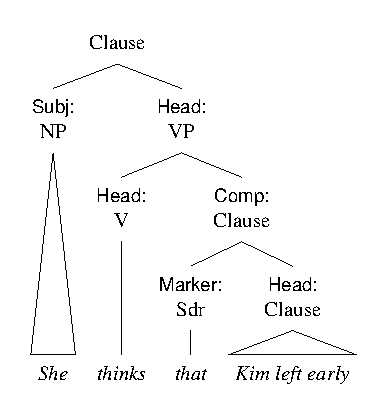
\includegraphics[width=0.55\linewidth]{figures/she thinks that kim left.pdf}
    \caption{অধীনীকরণ দেখানো বাক্যতাত্ত্বিক গাছ: \mention{She thinks that Kim left early}-এ \mention{that Kim left early} পরিপূরক হিসেবে কাজ করছে}\label{fig:sub-tree-sub-bn}
\end{figure}

অধীন গঠনে \mention{that} চিহ্ন হিসেবে দেখা যাচ্ছে, এটি লক্ষ করুন। \mention{that} নিজের কোনো গুচ্ছ projected করছে না; এটি শুধু অধীন উপবাক্যের শুরু চিহ্নিত করছে। \term{চিহ্নক} (\term{marker}, Mk) হলো এমন এক ধরনের নির্ভরশীল অংশ, যা প্রধান অংশটি বড় কাঠামোর সঙ্গে ব্যাকরণগতভাবে কীভাবে যুক্ত, তা দেখায়।

বিষয়বস্তু উপবাক্য বড় কাঠামোর ভেতরে নানা ভাবে কাজ করতে পারে।

\ea \label{ex:content-funcs-bn}
    \ea \gll I suspect {\ob}that he left{\cb}.\\
        I সন্দেহ-করা-PRS Sdr he চলে-যাওয়া-PST\\
    \glt \trans{আমার ধারণা, সে চলে গেছে।} [VP-র ভেতরে]
    \ex \gll The fact {\ob}that he left{\cb} is clear.\\
        DEF তথ্য Sdr he চলে-যাওয়া-PST হওয়া-PRS স্পষ্ট\\
    \glt \trans{সে চলে গেছে--এই তথ্য স্পষ্ট।} [NP-র ভেতরে]
    \ex \gll I'm glad {\ob}that he left{\cb}.\\
        I-হওয়া খুশি Sdr he চলে-যাওয়া-PST\\
    \glt \trans{সে চলে গেছে বলে আমি খুশি।} [AdjP-র ভেতরে]
    \ex \gll We can proceed provided {\ob}that he left{\cb}.\\
        we পারা-PRS এগোনো provided Sdr he চলে-যাওয়া-PST\\
    \glt \trans{সে যদি চলে গিয়ে থাকে, আমরা এগোতে পারি।} [PP-র ভেতরে]
    \ex \gll Whether or not he left is unclear.\\
        whether or not he চলে-যাওয়া-PST হওয়া-PRS অস্পষ্ট\\
    \glt \trans{সে চলে গেছে কি না, তা অস্পষ্ট।} [কর্তা]
    \ex \gll It's unclear whether or not he left.\\
        it-হওয়া অস্পষ্ট whether or not he চলে-যাওয়া-PST\\
    \glt \trans{সে চলে গেছে কি না, তা অস্পষ্ট।} [extraposed কর্তা]
    \z
\z

ঘোষণামূলক বিষয়বস্তু উপবাক্যে চিহ্নক, অর্থাৎ অধীনসূচক \mention{that}, উপবাক্যের কাজ অনুযায়ী বাধ্যতামূলক, ঐচ্ছিক, অথবা নিষিদ্ধ হতে পারে।
\ea\label{ex:marker-need-bn}
    \ea \gll That Kim left surprised no one.\\
        Sdr Kim চলে-যাওয়া-PST অবাক-করা-PST কেউ-না\\
    \glt \trans{কিম চলে গেছে--এতে কেউ অবাক হয়নি।} [বাধ্যতামূলক]
    \ex \gll I know that Kim left.\\
        I জানা-PRS Sdr Kim চলে-যাওয়া-PST\\
    \glt \trans{আমি জানি যে কিম চলে গেছে।} [ঐচ্ছিক]
    \ex \gll *We left before that Kim arrived.\\
        *we চলে-যাওয়া-PST before Sdr Kim আসা-PST\\
    \glt \trans{উদ্দিষ্ট অর্থ: কিম আসার আগে আমরা চলে গিয়েছিলাম। ইংরেজিতে এখানে \mention{that} ব্যবহার করা যায় না।} [*; অগ্রহণযোগ্য]
\z
\z
(\ref{ex:marker-need-bn}a)-এর মতো কর্তা-উপবাক্যে চিহ্নক সব সময় দরকার। পরিপূরক হিসেবে কাজ করলে ঘোষণামূলক উপবাক্যে (b)-এর মতো চিহ্নক সাধারণত থাকতে পারে বা না-ও থাকতে পারে। বড় ব্যতিক্রম হলো (c)-এর মতো PP-র ভেতরে পরিপূরক হিসেবে কাজ করা।

\label{sec:sub-interrog-bn}

প্রশ্নমূলক বিষয়বস্তু উপবাক্য আকর্ষণীয়, কারণ প্রধান প্রশ্ন-উপবাক্য থেকে এর বাক্যতত্ত্ব আলাদা। প্রধান উপবাক্যের মৌলিক প্রশ্ন \mention{Did she accept?}-এর মতো কর্তা ও সহায়ক ক্রিয়ার উলটক্রমে চেনা যায়। কিন্তু অধীন সংস্করণে \mention{whether} বা \mention{if} প্রশ্নত্ব চিহ্নিত করে।

\ea মৌলিক প্রশ্ন-উপবাক্য\label{ex:int-sub-bn}
    \ea \gll Did she accept?\\
        AUX she গ্রহণ-করা\\
    \glt \trans{সে কি গ্রহণ করেছিল?} [প্রধান, উলটক্রম]
    \ex \gll I wonder {\ob}whether she accepted{\cb}.\\
        I ভাবা-PRS whether she গ্রহণ-করা-PST\\
    \glt \trans{সে গ্রহণ করেছিল কি না, তা আমি ভাবছি।} [অধীন]
    \z
\z
\ea কেন্দ্রীভূত প্রশ্ন-উপবাক্য
    \ea \gll How did we get here?\\
        how AUX we আসা এখানে\\
    \glt \trans{আমরা এখানে কীভাবে এলাম?} [প্রধান, উলটক্রম]
    \ex \gll I wonder {\ob}how we got here{\cb}.\\
        I ভাবা-PRS how we আসা-PST এখানে\\
    \glt \trans{আমরা এখানে কীভাবে এলাম, তা আমি ভাবছি।} [অধীন]
    \z
\z
ইংরেজি শিক্ষার্থীদের জন্য এই পার্থক্য কঠিন। প্রাথমিক শিক্ষার্থী প্রায়ই কোনো উলটক্রম না করে প্রধান প্রশ্ন বানায়। অভিজ্ঞ শিক্ষার্থী উলটক্রম শেখার পর তা সব জায়গায় লাগিয়ে অধীন প্রশ্ন ভুল করে। এই পার্থক্য স্বচ্ছন্দে ব্যবহারের জন্য বেশ উচ্চ দক্ষতা দরকার।

তবু প্রধান প্রশ্ন ও অধীন প্রশ্নের কাঠামোগত দূরত্ব একটু একটু করে কমছে। উলটক্রম ধীরে ধীরে ছড়াচ্ছে। লেখায় উলটক্রমযুক্ত প্রশ্নমূলক বিষয়বস্তু উপবাক্য এখনও বিরল, কিন্তু (\ref{ex:non-inverted-interrogative-bn})-এর মতো উদাহরণ কথায় বেশ সাধারণ হয়ে উঠছে। কয়েকশো বছর পরে সব প্রশ্নে উলটক্রম মানক হয়ে যেতে পারে, আর চিহ্নক ঐচ্ছিক হতে পারে। আমি অপেক্ষা করব না।

\ea\label{ex:non-inverted-interrogative-bn}
\gll We need a story of {\ob}how did we get here{\cb}.\\
    we দরকার-PRS a গল্প of how AUX we আসা এখানে\\
\glt \trans{আমরা এখানে কীভাবে এলাম, সে বিষয়ে একটি গল্প আমাদের দরকার।}
\z
কিন্তু এখনকার ইংরেজিতে মৌলিক প্রশ্নমূলক বিষয়বস্তু উপবাক্যে \mention{whether} বা \mention{if}-এর মতো চিহ্নক প্রায় সব সময় দরকার। নইলে বেশির ভাগ ক্ষেত্রে তা চিহ্নকহীন ঘোষণামূলক উপবাক্য থেকে আলাদা করা যায় না।

\subsubsection*{mandative নির্মাণ}

অধীন গঠনের একটি বিশেষ উপধরন হলো \term{mandative নির্মাণ}। এটি দাবি, নির্দেশ, বা প্রয়োজনীয়তা বোঝানো বিধেয়ের সঙ্গে দেখা যায়।

\ea \label{ex:mandative-bn}
    \ea \gll It is essential {\ob}that he be there{\cb}.\\
        it হওয়া-PRS অপরিহার্য Sdr he থাকা-PLAIN সেখানে\\
    \glt \trans{তার সেখানে থাকা অপরিহার্য।} [বর্তমান subjunctive]
    \ex \gll It is essential {\ob}that he should be there{\cb}.\\
        it হওয়া-PRS অপরিহার্য Sdr he should থাকা সেখানে\\
    \glt \trans{তার সেখানে থাকা উচিত--এটি অপরিহার্য।} [should]
    \ex \gll It is essential {\ob}that he is there{\cb}.\\
        it হওয়া-PRS অপরিহার্য Sdr he থাকা-PRS সেখানে\\
    \glt \trans{সে সেখানে আছে--এটি অপরিহার্য।} [indicative]
    \z
\z
\term{বর্তমান subjunctive} (\term{present subjunctive}) রূপে ক্রিয়ার plain form ব্যবহৃত হয়। এখানে \enquote{subjunctive} মানে যে বাক্যটি অবাস্তব বা counterfactual, তা নয়। ইংরেজি \mention{that he be there}-এ গুরুত্বপূর্ণ হলো দাবি বা প্রয়োজনের প্রেক্ষিতে \mention{be} plain form হিসেবে এসেছে। \mention{should} রূপ অন্তত আগে ব্রিটিশ ইংরেজিতে বেশি প্রচলিত ছিল। আমেরিকান ইংরেজি বর্তমান subjunctive বেশি পছন্দ করে। \term{indicative} (\term{indicative}) রূপে সাধারণ tense-inflected form ব্যবহৃত হয়।

এতে দেখা যায়, অধীন উপবাক্যের ভেতরেও সূক্ষ্ম অর্থপার্থক্য এবং আঞ্চলিক পছন্দ থাকতে পারে। শিক্ষণ-দৃষ্টিকোণ থেকে বলার মতো বিষয় হলো: indicative রূপ, বিশেষত অনানুষ্ঠানিক প্রেক্ষিতে, বাড়ছে; কিন্তু আনুষ্ঠানিক লেখায় বর্তমান subjunctive এখনও মানক।

\begin{tblsframedsymbol}{বোঝাপড়া যাচাই: ধারক ও অধীন উপবাক্য}{test}
কাঠামোগত সম্পর্কগুলি খুঁজুন।
\begin{itemize}[noitemsep, leftmargin=*]
    \item \mention{I know that she thinks that he left}-এ প্রধান উপবাক্য, ধারক উপবাক্য, এবং অধীন উপবাক্য খুঁজুন।
    \item \mention{She asked whether he left}-এ উলটক্রম নেই, কিন্তু \mention{Did he leave?}-এ আছে কেন, তা ব্যাখ্যা করুন।
    \item mandative নির্মাণ খুঁজুন: \mention{It's important that he be careful} এবং \mention{It's important that he is careful}.
\end{itemize}
এই সম্পর্কগুলি বুঝলে অর্থ কীভাবে বাক্যতাত্ত্বিক কাঠামো থেকে তৈরি হয়, তা ভালো দেখা যায়।
\end{tblsframedsymbol}

\subsection{তুলনামূলক উপবাক্য}

finite অধীন উপবাক্যের দ্বিতীয় প্রধান ধরন হলো তুলনামূলক উপবাক্য। তুলনামূলক উপবাক্য (\ref{ex:comparative-intro-bn})-এর মতো তুলনা সম্পূর্ণ করে।

\ea \label{ex:comparative-intro-bn}
    \ea \gll The ice was thicker than {\ob}we expected{\cb}.\\
        DEF বরফ হওয়া-PST বেশি-পুরু than we আশা-করা-PST\\
    \glt \trans{বরফ আমাদের প্রত্যাশার চেয়ে বেশি পুরু ছিল।}
    \ex \gll She writes faster than {\ob}she speaks{\cb}.\\
        she লেখা-PRS বেশি-দ্রুত than she বলা-PRS\\
    \glt \trans{সে কথা বলার চেয়ে দ্রুত লেখে।}
    \ex \gll It doesn't cost as much as {\ob}I'd thought{\cb}.\\
        it NEG খরচ-হওয়া-PRS as বেশি as I-ভাবা-PST\\
    \glt \trans{আমি যতটা ভেবেছিলাম, এর খরচ তত বেশি নয়।}
    \z
\z
তুলনামূলক উপবাক্যকে বিষয়বস্তু উপবাক্য থেকে আলাদা করে যে বৈশিষ্ট্যটি, তা হলো এতে ellipsis থাকে। প্রসঙ্গ থেকে উদ্ধারযোগ্য উপাদান বাদ পড়ে। (\ref{ex:comparative-ellipsis-bn})-এ ... এই বাদ পড়া বোঝায়।\footnote{আগের অধ্যায়ে gap পরিচয় করানো হয়েছে। gap গাছের ভেতরে একটি কাঠামোগত অবস্থান। ellipsis-এ থাকা উপাদান প্রসঙ্গ থেকে অর্থগতভাবে উদ্ধার করা যায়, কিন্তু তা বাক্যতাত্ত্বিক উপাদান হিসেবে থাকে না।}

\ea \label{ex:comparative-ellipsis-bn}
    \ea \gll Kim read more books than {\ob}Pat read ...{\cb}.\\
        Kim পড়া-PST বেশি বই-PL than Pat পড়া-PST ...\\
    \glt \trans{প্যাট যত বই পড়েছিল, কিম তার চেয়ে বেশি বই পড়েছিল।}
    \ex \gll Kim read more books than {\ob}Pat did ...{\cb}.\\
        Kim পড়া-PST বেশি বই-PL than Pat AUX.PST ...\\
    \glt \trans{কিম প্যাটের চেয়ে বেশি বই পড়েছিল।}
    \ex \gll Kim read more books than {\ob}Pat{\cb}.\\
        Kim পড়া-PST বেশি বই-PL than Pat\\
    \glt \trans{কিম প্যাটের চেয়ে বেশি বই পড়েছিল।}
    \z
\z

প্রথম দুটি রূপে ellipsis দেখা যায়। (b)-তে \mention{read} পুনরাবৃত্তির বদলে VP pro-form \mention{did} এসেছে। তৃতীয় (c)-তে \mention{Pat} উপবাক্যের পরিপূরক নয়; এটি NP পরিপূরক। তিনটির মূল অর্থ একই।

বেশির ভাগ ellipsis-এর বিপরীতে, তুলনামূলক উপবাক্যে বাদ পড়া তথ্য স্পষ্ট করে বললে বাক্য অগ্রহণযোগ্য হয়। যেমন *\mention{Kim read more books than Pat read 20 books} বা *\mention{It's not as deep as it is 20 cm wide} বলা যায় না। ellipsis এই উপবাক্য-ধরনের কেন্দ্রীয় অংশ। তুলনামূলক উপবাক্যের কাঠামো চিত্র~\ref{fig:comp-tree-bn}-এ আছে।

\begin{figure}
    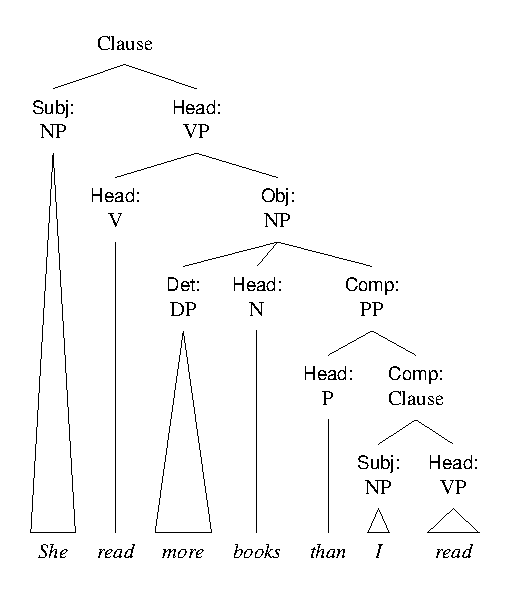
\includegraphics[width=0.7\linewidth]{figures/she read more books than I read.pdf}
    \caption{ellipsis-সহ তুলনামূলক উপবাক্য দেখানো বাক্যতাত্ত্বিক গাছ}\label{fig:comp-tree-bn}
\end{figure}

তুলনার ধরন অনুযায়ী তুলনামূলক উপবাক্য \mention{than} বা \mention{as}-যুক্ত PP-র ভেতরে পরিপূরক হিসেবে কাজ করে।

\ea \label{ex:comp-markers-bn}
    \ea \gll Kim is taller than {\ob}Pat is{\cb}.\\
        Kim হওয়া-PRS বেশি-লম্বা than Pat হওয়া-PRS\\
    \glt \trans{কিম প্যাটের চেয়ে লম্বা।} [অসমতা]
    \ex \gll Kim is as tall as {\ob}Pat is{\cb}.\\
        Kim হওয়া-PRS as লম্বা as Pat হওয়া-PRS\\
    \glt \trans{কিম প্যাটের মতোই লম্বা।} [সমতা\footnote{এখানে \enquote{\term{সমতা}} শব্দটি একটু বিভ্রান্তিকর হতে পারে। এই উদাহরণের অর্থ কিম অন্তত প্যাটের মতো লম্বা; কিম আরও লম্বা হতে পারে।}]
    \z
\z
(\ref{ex:comp-markers-bn}a)-এর \mention{than} অসমতা দেখায়, আর (b)-এর \mention{as} সমতা চিহ্নিত করে। প্রথম \mention{as} একটি adverb। \mention{as tall} একটি AdjP, এবং তার ভেতরে \mention{as} modifier হিসেবে কাজ করে। দ্বিতীয় \mention{as} preposition।

ইংরেজি শিক্ষার্থীদের জন্য তুলনামূলক উপবাক্যে কয়েকটি অসুবিধা আছে।
\begin{itemize}[noitemsep]
    \item কী, কখন, কতটা বাদ দেওয়া যায়, তা বোঝা।
    \item সমতা ও অসমতার আলাদা ধরন আয়ত্ত করা।
    \item একাধিক উপাদান জড়ানো জটিল তুলনা সামলানো।
\end{itemize}

ভালো খবর হলো তুলনামূলক উপবাক্য বেশ নিয়মিত ছক মেনে চলে। বেশি জটিল কাঠামোতে যাওয়ার আগে শিক্ষার্থীরা \mention{taller than} `...-এর চেয়ে লম্বা' বা \mention{as tall as} `অন্তত ...-এর মতো লম্বা' ধরনের মৌলিক ছক শিখতে পারে।

\section{সমপদী সংযোগ}\label{sec:coordination-bn}

অধীনীকরণ উপবাক্যগুলির মধ্যে নির্ভরতার সম্পর্ক তৈরি করে; \term{সমপদী সংযোগ} একই বাক্যতাত্ত্বিক মর্যাদার উপাদান যুক্ত করে। এই ব্যবস্থার কেন্দ্রে আছে ছোট, closed word class: \term{সমপদী-সংযোগক} (\term{coordinator}, Crd)। প্রধান সদস্য \mention{and}, \mention{or}, \mention{but}; তিনটি গণনা করতেও তিনটিই লাগে। অধীনসূচকের মতো সমপদী-সংযোগকও চিহ্নক হিসেবে কাজ করে।

এখানে \term{সমপদী সংযোগ} মানে শুধু ভাব স্বাভাবিকভাবে জুড়ে যাচ্ছে নয়। বাংলায় \enquote{যোগ}, \enquote{সংযোগ}, বা \enquote{সমন্বয়} কথাগুলি কথাবার্তার ধারাবাহিকতা বা পরিকল্পনার মিলও মনে করাতে পারে। এই অধ্যায়ে দরকার একটি কাঠামোগত সম্পর্ক: দুটি বা তার বেশি উপাদান একই বাক্যতাত্ত্বিক মর্যাদায় থাকে, এবং কোনোটি পুরো গঠনের প্রধান নয়। এই কথা না ধরলে সমপদী সংযোগকে শুধু তালিকা বা বক্তব্য-প্রবাহের যোগ হিসেবে ভুল বোঝা সহজ।

নিচের উদাহরণগুলি দেখুন।

\ea \label{ex:coord-basic-bn}
    \ea \gll {\ob}Jane is a good teacher{\cb} {\ob}and her students really like her{\cb}.\\
        Jane হওয়া-PRS a ভালো শিক্ষক and her ছাত্র-PL সত্যিই পছন্দ-করা-PRS her\\
    \glt \trans{জেন ভালো শিক্ষক এবং তার ছাত্ররা তাকে সত্যিই পছন্দ করে।}
    \ex \gll They offered us a choice of {\ob}red wine{\cb}, {\ob}white wine{\cb}, {\ob}or beer{\cb}.\\
        they দেওয়া-PST us a পছন্দ of লাল মদ সাদা মদ or বিয়ার\\
    \glt \trans{তারা আমাদের লাল মদ, সাদা মদ, অথবা বিয়ারের একটি পছন্দ দিয়েছিল।}
    \ex \gll Her assistant is {\ob}very young{\cb} {\ob}but a quick learner{\cb}.\\
        her সহকারী হওয়া-PRS খুব তরুণ but a দ্রুত শিক্ষার্থী\\
    \glt \trans{তার সহকারী খুব তরুণ, কিন্তু দ্রুত শেখে।}
    \z
\z
এই উদাহরণগুলিতে সংশ্লিষ্ট উপাদানগুলি \term{সমপদী উপাদান} (\term{coordinate}) হিসেবে কাজ করছে। এই কাজটি (\ref{ex:coord-basic-bn}a)-এর মতো উপবাক্য, (b)-এর মতো NP বা অন্য গুচ্ছ, এবং আরও বিরলভাবে (c)-এর AdjP ও NP-র মতো মিশ্র শ্রেণি দিয়ে বাস্তবায়িত হতে পারে। সমপদী-সংযোগক সাধারণত আলাদা সম্পর্ক প্রকাশ করে: \mention{and} যোগ, \mention{or} বিকল্প, \mention{but} বৈপরীত্য।

সমপদী সংযোগের আগের গঠনগুলির সঙ্গে বড় পার্থক্য হলো এখানে প্রধান নেই। কোনো সমপদী উপাদানই পুরো গঠনের প্রধান নয়। এই প্রধানহীনতা একটি সরল পরীক্ষায় দেখা যায়। অনেক ক্ষেত্রে পুরো সমপদী গঠনকে সমপদী উপাদানগুলির একটির সঙ্গে বদলে দেওয়া যায়।

\ea \label{ex:coord-replace-bn}
    \ea \gll Her assistant is very young.\\
        her সহকারী হওয়া-PRS খুব তরুণ\\
    \glt \trans{তার সহকারী খুব তরুণ।}
    \ex \gll Her assistant is a quick learner.\\
        her সহকারী হওয়া-PRS a দ্রুত শিক্ষার্থী\\
    \glt \trans{তার সহকারী দ্রুত শেখে।}
    \z
\z
(\ref{ex:coord-replace-bn}a) ও (b) দুটিই (\ref{ex:coord-basic-bn}c)-এর ব্যাকরণসম্মত বিকল্প। এটি \mention{very young}-এর মতো প্রধানযুক্ত গঠনের থেকে আলাদা। সে ক্ষেত্রে প্রধান অংশ একা ব্যবহার করা যায় (\mention{she's young}), কিন্তু নির্ভরশীল অংশ একা নয় (*\mention{she's very})। সমপদী সংযোগের কাঠামো চিত্র~\ref{fig:coord-basic-bn}-এ আছে।

\begin{figure}
    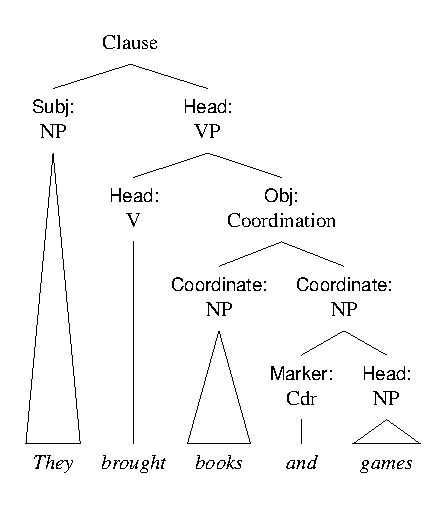
\includegraphics[width=0.65\linewidth]{figures/the brought books and games.pdf}
    \caption{চিহ্নকসহ মৌলিক সমপদী সংযোগ: \mention{They brought books and games}}\label{fig:coord-basic-bn}
\end{figure}

\subsection{সমপদী সংযোগের বৈশিষ্ট্য}

তিনটি গুরুত্বপূর্ণ বৈশিষ্ট্য সমপদী সংযোগকে অন্য গঠন থেকে আলাদা করে।

সমপদী উপাদানের সংখ্যায় ব্যাকরণগত সীমা নেই। \mention{but} ব্যতিক্রম।

\ea \label{ex:coord-multiple-bn}
\gll Nothing noble, sublime, profound, delicate, tasteful or even decent can find a place.\\
    কিছুই মহৎ ঊর্ধ্ব গভীর সূক্ষ্ম রুচিসম্পন্ন or এমনকি শোভন পারা-PRS খুঁজে-পাওয়া a স্থান\\
\glt \trans{মহৎ, ঊর্ধ্ব, গভীর, সূক্ষ্ম, রুচিসম্পন্ন, এমনকি শোভন কিছুই স্থান পায় না।}
\z

সমপদী উপাদানগুলি কার্যগতভাবে মিল থাকতে হবে। একা ব্যবহৃত হলে তাদের একই কাজ করতে পারতে হবে।

\ea \label{ex:coordinate-function-bn}
    \ea \gll I'll be back next week or at the end of the month.\\
        I-FUT ফিরে-আসা আগামী সপ্তাহ or at DEF শেষ of DEF মাস\\
    \glt \trans{আমি আগামী সপ্তাহে বা মাসের শেষে ফিরব।} [সময়-সংশোধক]
    \ex \gll *We're leaving Rome and next week.\\
        *we-PRS ছাড়া Rome and আগামী সপ্তাহ\\
    \glt \trans{উদ্দিষ্ট কাঠামো ইংরেজিতে অস্বাভাবিক। \mention{Rome} object, কিন্তু \mention{next week} adjunct।} [*; object ও adjunct]
    \z
\z

বিস্তৃত সমপদী উপাদান, অর্থাৎ সমপদী-সংযোগকসহ সমপদী উপাদান, সামনে সরানো যায় না।

\ea \label{ex:coord-front-bn}
    \ea \gll They attended but they aren't members.\\
        they উপস্থিত-থাকা-PST but they NEG-হওয়া-PRS সদস্য-PL\\
    \glt \trans{তারা উপস্থিত ছিল, কিন্তু সদস্য নয়।}
    \ex \gll *But they aren't members, they attended.\\
        *but they NEG-হওয়া-PRS সদস্য-PL they উপস্থিত-থাকা-PST\\
    \glt \trans{উদ্দিষ্ট অর্থ: তারা উপস্থিত ছিল, কিন্তু সদস্য নয়। ইংরেজিতে \mention{but}-সহ বিস্তৃত সমপদী উপাদান এভাবে সামনে আনা যায় না।} [*]
    \z
\z

\subsection{বাক্যের শুরুতে সমপদী-সংযোগক সম্পর্কে}

\mention{and} বা \mention{but}-এর মতো সমপদী-সংযোগক দিয়ে বাক্য শুরু করা যাবে না--এমন নিয়মধর্মী উপদেশ আছে। কিন্তু এই নিষেধ ইংরেজি ব্যাকরণ বা বাস্তব ব্যবহারের উপর দাঁড়ায় না। ইংরেজির ইতিহাস জুড়েই দক্ষ লেখকেরা বাক্যের শুরুতে সমপদী-সংযোগক ব্যবহার করেছেন। এই বইয়ের এই অধ্যায় এবং অন্য অধ্যায়েও অনেক উদাহরণ পাবেন। তবে বাক্যের শুরুতে থাকা সমপদী-সংযোগক সেই বাক্যকে আগের বাক্যের সঙ্গে সংকীর্ণ অর্থে সমপদী সংযোগে বাঁধতে পারে না। (\ref{ex:coord-front-bn})-এর সামনে-সরানোর সীমা মনে করুন। বরং এটি \term{বক্তব্য-সংযোগক} (\term{discourse connector}) হিসেবে কাজ করে, নতুন বাক্য আগের কথার সঙ্গে কীভাবে যুক্ত তা দেখায়।

বাংলা পাঠকের জন্য এ জায়গায় ভুল বোঝা সহজ। বাংলা গদ্যে \enquote{আর}, \enquote{কিন্তু}, \enquote{তবে}, \enquote{অথচ} বাক্য শুরুতে বক্তব্য-সংযোগক হিসেবে খুব স্বাভাবিক। কিন্তু এই অধ্যায়ের সমপদী সংযোগ একটি বাক্যতাত্ত্বিক কাঠামোর ভেতরে একই মর্যাদার উপাদান যুক্ত করা। আসল সীমা শুধু শৈলগত। যেকোনো উপকরণের মতো বাক্য-শুরুর সংযোগক বেশি ব্যবহার করলে লেখা একঘেয়ে হয়। সাবধানে ব্যবহার করলে তা বক্তব্যের প্রবাহ সামলায় এবং পাঠ্যের সম্পর্ক চিহ্নিত করে।

\subsection{সমপদী সংযোগের ধরন}

সবচেয়ে সরল পার্থক্য হলো \term{সমমিত সমপদী সংযোগ} (\term{symmetric coordination}) এবং \term{অসমমিত সমপদী সংযোগ} (\term{asymmetric coordination})। সমমিত সমপদী সংযোগে সমপদী উপাদানের ক্রম অর্থ বদলায় না; অসমমিত সমপদী সংযোগে বদলায়।

\ea \label{ex:coord-sym-bn}
    \ea \gll I was hungry and tired.\\
        I হওয়া-PST ক্ষুধার্ত and ক্লান্ত\\
    \glt \trans{আমি ক্ষুধার্ত ও ক্লান্ত ছিলাম।} [সমমিত]
    \ex \gll I got up and had breakfast.\\
        I ওঠা-PST and খাওয়া-PST সকালের-খাবার\\
    \glt \trans{আমি উঠলাম এবং সকালের খাবার খেলাম।} [অসমমিত]
    \z
\z
(\ref{ex:coord-sym-bn}a)-তে সমপদী উপাদানের ক্রম পাল্টালেও অর্থ বদলায় না। কিন্তু (b)-তে ক্রম সময়গত ধারাবাহিকতা বোঝায়। ওঠা সকালের খাবারের আগে ঘটেছে।

\term{বণ্টনমূলক সমপদী সংযোগ} (\term{distributive coordination}) এবং \term{সমষ্টিগত সমপদী সংযোগ} (\term{joint coordination})-ও আলাদা করা হয়।

\ea \label{ex:coord-dist-bn}
    \ea \gll Kim and Pat are fine players.\\
        Kim and Pat হওয়া-PRS ভালো খেলোয়াড়-PL\\
    \glt \trans{কিম ও প্যাট ভালো খেলোয়াড়।} [বণ্টনমূলক]
    \ex \gll Kim and Pat are a good pair.\\
        Kim and Pat হওয়া-PRS a ভালো জুটি\\
    \glt \trans{কিম ও প্যাট ভালো জুটি।} [সমষ্টিগত]
    \z
\z
(\ref{ex:coord-dist-bn}a)-তে ভালো খেলোয়াড় হওয়ার গুণটি কিম ও প্যাট প্রত্যেকের উপর আলাদাভাবে প্রযোজ্য। কিন্তু (b)-তে ভালো জুটি হওয়া দুইজনের উপর একত্রে প্রযোজ্য হলেই সত্য। একজন একা জুটি হতে পারে না।

\subsection{সমপদী সংযোগের চিহ্নায়ন}

সমপদী সংযোগ নানা ভাবে চিহ্নিত হতে পারে।
\begin{itemize}[noitemsep]
    \item সমপদী-সংযোগক ব্যবহার করে: \mention{red and blue}
    \item কোনো চিহ্নক না দিয়ে: \mention{red, white, blue}
    \item সমপদী-সংযোগক পুনরাবৃত্তি করে: \mention{red or white or blue}
    \item যুগ্ম চিহ্নক ব্যবহার করে: \mention{both red and blue}
\end{itemize}

সমপদী-সংযোগক সাধারণত যোগ (\mention{and}), বিকল্প (\mention{or}), এবং বৈপরীত্য (\mention{but}) প্রকাশ করে; কিন্তু অসমমিত সমপদী সংযোগে বাড়তি অর্থও পেতে পারে।

\ea \label{ex:coord-meaning-bn}
    \ea \gll Pay within a week and you'll get a discount.\\
        পরিশোধ-করা within a সপ্তাহ and you-FUT পাওয়া a ছাড়\\
    \glt \trans{এক সপ্তাহের মধ্যে পরিশোধ করলে ছাড় পাবে।} [শর্ত]
    \ex \gll Pay within a week or you'll lose the discount.\\
        পরিশোধ-করা within a সপ্তাহ or you-FUT হারানো DEF ছাড়\\
    \glt \trans{এক সপ্তাহের মধ্যে পরিশোধ না করলে ছাড় হারাবে।} [নেতিবাচক শর্ত]
    \z
\z

\begin{tblsframedsymbol}{ছক চেনা: সমপদী সংযোগ না অধীনীকরণ?}{test}
নিচের গঠনগুলি আলাদা করতে নির্ণায়ক পরীক্ষা ব্যবহার করুন।
\begin{itemize}[noitemsep, leftmargin=*]
    \item \mention{She thinks that he left} এবং \mention{She left and he stayed}: কোনটি এক উপবাক্যকে অন্যটির ভেতরে বসায়, আর কোনটি একই মর্যাদার দুটি উপবাক্য যুক্ত করে?
    \item \mention{Although it rained, we went} এবং \mention{It rained but we went}: কোনটি নির্ভরতার স্তরবিন্যাস দেখায়, আর কোনটি সমমর্যাদা দেখায়?
    \item \mention{*But we went, it rained} এবং \mention{Although it rained, we went}: সামনে-সরানো কাঠামো সম্পর্কে কী দেখায়?
\end{itemize}
এই পরীক্ষাগুলি স্তরযুক্ত সন্নিবেশ এবং সমমর্যাদার উপাদান-সংযোগ আলাদা করতে সাহায্য করে।
\end{tblsframedsymbol}

সমপদী-সংযোগক পরিচয় করানো হয়ে গেলে, interjection ছাড়া ইংরেজির প্রধান lexical category সবই দেখা হলো। সেই সঙ্গে উপবাক্যের ভেতরে তাদের প্রধান বাক্যতাত্ত্বিক কাজও দেখা হয়েছে।

\subsection{সমপদী সংযোগের কাঠামো}

উপাদানগুলিকে সমপদীভাবে যুক্ত করলে তাদের একই বাক্যতাত্ত্বিক কাজ ভাগ করে নিতে হবে। অর্থাৎ পরিপূরকগুলিকে পরিপূরকের সঙ্গে, সংশোধকগুলিকে সংশোধকের সঙ্গে যুক্ত করা যায়; কিন্তু পরিপূরক ও সংশোধককে একসঙ্গে সমপদী করা যায় না। তুলনা করুন।

\ea \label{ex:coord-function-bn}
    \ea \gll We listened {\ob}to the teacher{\cb} {\ob}and the students{\cb}.\\
        we শোনা-PST to DEF শিক্ষক and DEF ছাত্র-PL\\
    \glt \trans{আমরা শিক্ষক ও ছাত্রদের কথা শুনলাম।} [পরিপূরক]
    \ex \gll We listened {\ob}Monday{\cb} and {\ob}Tuesday{\cb}.\\
        we শোনা-PST সোমবার and মঙ্গলবার\\
    \glt \trans{আমরা সোমবার ও মঙ্গলবার শুনলাম।} [সংশোধক]
    \ex \gll *We listened {\ob}to the teachers{\cb} and {\ob}Monday{\cb}.\\
        *we শোনা-PST to DEF শিক্ষক-PL and সোমবার\\
    \glt \trans{উদ্দিষ্ট কাঠামো ইংরেজিতে অস্বাভাবিক। \mention{to the teachers} পরিপূরক, কিন্তু \mention{Monday} সংশোধক।} [*; কাজ মিশ্রিত]
    \z
\z
যে উপাদানগুলি সমপদীভাবে যুক্ত হয়, অর্থাৎ \term{সমপদী উপাদান}, তারা প্রধান গুচ্ছ-ধরনের যেকোনো জায়গায় আসতে পারে: noun, verb, adjective, preposition, বড় গুচ্ছ বা উপবাক্য। গুরুত্বপূর্ণ হলো তারা বড় কাঠামোর ভেতরে একইভাবে কাজ করে।

\subsection{চিহ্নিত ও অচিহ্নিত সমপদী সংযোগ}

সমপদী সংযোগে স্পষ্ট সমপদী-সংযোগক থাকতে পারে, আবার না-ও থাকতে পারে। সমপদী-সংযোগক না থাকলে তাকে \term{সংযোগকহীন সমপদী সংযোগ} (\term{asyndetic coordination}) বলা হয়।

\ea \label{ex:coord-marking-bn}
    \ea \gll She brought {\ob}games{\cb}, {\ob}stories{\cb}, {\ob}songs{\cb}.\\
        she আনা-PST খেলা-PL গল্প-PL গান-PL\\
    \glt \trans{সে খেলা, গল্প, গান এনেছিল।} [সংযোগকহীন]
    \ex \gll She brought {\ob}games{\cb}, {\ob}stories{\cb}, and {\ob}songs{\cb}.\\
        she আনা-PST খেলা-PL গল্প-PL and গান-PL\\
    \glt \trans{সে খেলা, গল্প, এবং গান এনেছিল।} [সংযোগকসহ]
    \z
\z
একটি সমপদী-সংযোগকযুক্ত সরল সমপদী সংযোগের পাশাপাশি \term{যুগ্ম-চিহ্নক সমপদী সংযোগ} (\term{correlative coordination}) আছে। এতে একাধিক সমপদী উপাদানে চিহ্নক দেখা যায়।

\ea \label{ex:coord-correlative-bn}
    \ea \gll {\ob}Both{\cb} tired {\ob}and{\cb} hungry\\
        both ক্লান্ত and ক্ষুধার্ত\\
    \glt \trans{ক্লান্তও, ক্ষুধার্তও}
    \ex \gll {\ob}Either{\cb} now {\ob}or{\cb} never\\
        either এখন or কখনো-না\\
    \glt \trans{এখন, না হলে কখনো নয়}
    \ex \gll {\ob}Neither{\cb} simple {\ob}nor{\cb} easy\\
        neither সরল nor সহজ\\
    \glt \trans{না সরল, না সহজ}
    \z
\z

\subsection{স্তরযুক্ত সমপদী সংযোগ}

সমপদী উপাদান নিজেই সমপদী সংযোগ ধারণ করতে পারে। একে স্তরযুক্ত সমপদী সংযোগ বলা যায়। নিচের উদাহরণটি ভাবুন।

\ea \label{ex:coord-layered-bn}
\gll The story was {\ob}short and sweet{\cb} but {\ob}complex and thought-provoking{\cb}.\\
    DEF গল্প হওয়া-PST ছোট and মধুর but জটিল and ভাবনা-জাগানো\\
\glt \trans{গল্পটি ছোট ও মধুর ছিল, কিন্তু জটিল এবং ভাবনা-জাগানো।}
\z
এখানে \mention{but} দিয়ে যুক্ত দুটি প্রধান সমপদী উপাদান আছে। কিন্তু তাদের প্রত্যেকের ভেতরেই \mention{and}-যুক্ত সমপদী সংযোগ আছে। এমন স্তরায়ন ভাবগুলির জটিল সম্পর্ক প্রকাশ করতে দেয়, কিন্তু কাঠামো স্পষ্ট রাখে। স্তরযুক্ত কাঠামো চিত্র~\ref{fig:coord-layered-bn}-এ আছে।

\begin{figure}
    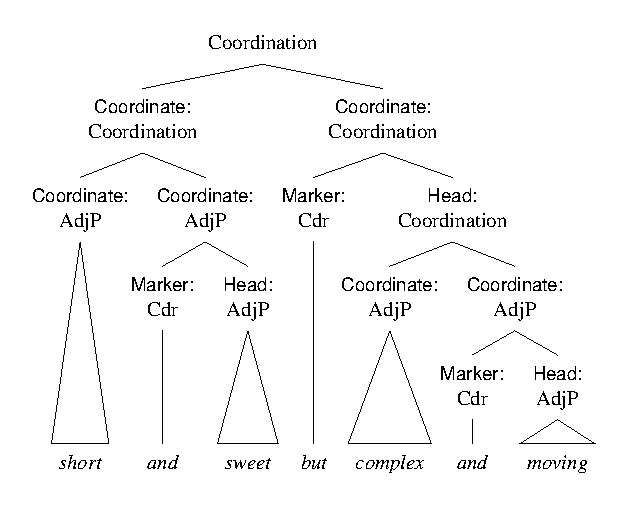
\includegraphics[width=0.9\linewidth]{figures/short and sweet but complex and moving.pdf}
    \caption{স্তরযুক্ত সমপদী সংযোগ: \mention{short and sweet but complex and moving}}\label{fig:coord-layered-bn}
\end{figure}

\subsection{বিশেষ সমপদী সংযোগ}

একটি বিশেষভাবে আকর্ষণীয় সমপদী সংযোগ তুলনামূলক গঠনে দেখা যায়।

\ea \label{ex:coord-comp-bn}
    \ea \gll He's as tall as {\ob}or taller than{\cb} his brother.\\
        he-হওয়া as লম্বা as or বেশি-লম্বা than his ভাই\\
    \glt \trans{সে তার ভাইয়ের মতোই লম্বা, অথবা তার চেয়েও লম্বা।}
    \ex \gll She writes more {\ob}but understands less{\cb} than before.\\
        she লেখা-PRS বেশি but বোঝা-PRS কম than আগে\\
    \glt \trans{সে আগের চেয়ে বেশি লেখে, কিন্তু কম বোঝে।}
    \z
\z
এই গঠনগুলিতে প্রায়ই সমপদী উপাদান এবং তারা যে অংশ ভাগ করে, তার মধ্যে জটিল সম্পর্ক থাকে। এগুলি ব্যাখ্যা করতে হলে সমপদী সংযোগ ও তুলনামূলক সম্পর্ক দুটোই বুঝতে হয়।

\begin{tblsframedsymbol}{দ্রুত আত্মপরীক্ষা: জটিল কাঠামো}{test}
স্তরযুক্ত গঠন বিশ্লেষণ করতে পারেন কি না, দেখে নিন।
\begin{itemize}[noitemsep, leftmargin=*]
    \item \mention{I know that she left and he stayed}-এ সব অধীনীকরণ সম্পর্ক ও সমপদী সংযোগ সম্পর্ক খুঁজুন।
    \item \mention{Both young and talented, she succeeded}-এ যুগ্ম চিহ্নক এবং সমপদীভাবে যুক্ত adjectives খুঁজুন।
    \item এই গঠনটি বিশ্লেষণ করুন: \mention{He's taller than I thought but shorter than his brother}.
\end{itemize}
এই জটিল ধরনগুলি বুঝলে দেখা যায়, অধীনীকরণ ও সমপদী সংযোগ কীভাবে একসঙ্গে অর্থ তৈরি করে।
\end{tblsframedsymbol}

\section{সারাংশ}

অধীনীকরণ ও সমপদী সংযোগ দুটিই ভাবকে যুক্ত করে, কিন্তু তারা বিপরীত কাঠামো ব্যবহার করে। অধীনীকরণ বসায়; সমপদী সংযোগ জোড়ে। ভালো লেখা দুটির ভারসাম্য রাখে। শিক্ষার্থী কী কাঠামো বানাতে চাইছে, আর কোথায় কাঠামোটি ভেঙে যাচ্ছে, তা বুঝতে পারলে আমরা শুধু \enquote{কিছু একটা অদ্ভুত} মনে করে থেমে থাকি না; সমস্যার নাম বলতে পারি। স্তর বেশি, তালিকা বেশি, যেখানে সমপদী-সংযোগক যথেষ্ট ছিল সেখানে অধীনসূচক এসেছে--এইভাবে।
